\documentclass[10pt,a4paper]{article}
\usepackage[utf8]{inputenc}
\usepackage[top=1in, bottom=1in, left=0.6in, right=0.6in]{geometry}
\usepackage{lipsum}
\usepackage{amsmath}
\usepackage{amsfonts}
\usepackage{amssymb}
\usepackage[hidelinks]{hyperref}
\usepackage{graphicx}
\usepackage[
backend=biber,
style=numeric,
doi=false,
url=false,
maxbibnames=9
]{biblatex}
\addbibresource{sysbio2018_blackboard.bib}

%\newcommand{\mymatrix}[1]{{\boldsymbol{#1}}}
\newcommand{\mymatrix}[1]{#1}
\newcommand{\myvector}[1]{{\boldsymbol{#1}}}
\newcommand{\fluxcone}{\mathcal{C}}
\newcommand{\stoichmat}{\mymatrix{S}}
\newcommand{\stoichmatint}{\mymatrix{S}_{\mathsf{int}}}

\date{March 2, 2018}
\title{\textbf{SysBio 2018}\\Innsbruck, Austria}
\author{Elad Noor}
\begin{document}
\maketitle
\tableofcontents

\section{Blackboard session: Metabolic Engineering}

\subsection{Introduction}
\subsubsection{Linear Programming (LP)}
Every Linear Programming problem can be converted to a canonical form that is:
\begin{eqnarray}
	\textsf{\textbf{Primal}}&&\nonumber\\
	\textsf{maximize}&\myvector{c}^\top\myvector{x}&\nonumber\\
	\textsf{subject to}&\mymatrix{A}\myvector{x} \leq \myvector{b}&\nonumber\\
	\textsf{and}&\myvector{x}\geq \myvector{0}&
\end{eqnarray}

Dual
\begin{eqnarray}
	\textsf{\textbf{Dual}}&&\nonumber\\
	\textsf{minimize}&\myvector{b}^\top\myvector{y}&\nonumber\\
	\textsf{subject to}&\mymatrix{A}^\top\myvector{y} \geq \myvector{c}&\nonumber\\
	\textsf{and}&\myvector{y}\geq 0&
\end{eqnarray}

Linear Programming problems can be solved very efficiently using established algorithms such as Simplex. Many good solvers exist for LP, including open source options such as glpk, CLP, and the internal R-project solver.

\subsubsection{Mixed-Integer Linear Programming (MILP)}
If a LP contains variables that can only have integer values (or in a more specific case, boolean values), the problem cannot be solved using the standard methods. In fate, MILP problems in general are NP-complete, i.e. computationally hard. The free solvers are typically not good enough for solving MILPs. Nevertheless, advanced commercial solvers such as CPLEX and Gurobi are quite efficient in solving even large MILPs in reasonable time, and provide free licenses for academics.

\subsection{Convex analysis of a metabolic flux cone}
The basic idea underlying most metabolic constraint-based models, is mass-balance combined with the steady-state assumption. Formally, given a stoichiometric matrix $\mymatrix{S}$, where rows represent metabolites and column represent reactions, and given a flux vector $\myvector{v}$, the rate of change in metabolite levels ($\myvector{c}$) is given by the equation.
\begin{eqnarray}\label{eq:dynamic-mass-balance}
	&\textsf{\textbf{Dynamic mass-balance}} &\nonumber\\
    &&\frac{d\myvector{c}}{dt} = \stoichmat \myvector{v}~~~~~~~~~~~~~~~~~~~~~~~~~~~~~~~~~~~~~
\end{eqnarray}
For the subset of rows in $\stoichmat$ that represent internal metabolites (e.g. intracellular metabolites) which is denoted $\stoichmatint$, the pseudo steady-state assumption states that their concentrations do not change over time.
\begin{eqnarray}\label{eq:pseudo-steady-state}
	&\textsf{\textbf{Pseudo steady-state}} &\nonumber\\
	&&\stoichmatint \myvector{v} = 0~~~~~~~~~~~~~~~~~~~~~~~~~~~~~~~~~~~~~
\end{eqnarray}
Note that external metabolites are not constrained in this way. For example, the concentration of extracellular glucose in the medium decreases gradually while cells are growing at steady-state. Therefore, pseudo steady-state flux solutions are contained within the null-space (or kernel) of $\stoichmatint$, i.e. $\myvector{v} \in \ker(\stoichmatint)$.

\subsubsection{The flux cone}
Typically, many of the reactions in our model will be considered irreversible, due to thermodynamic constraints (and we will elaborate on this topic in section \ref{sec:thermodynamics}). Therefore, a subset of the fluxes will be constrained to be positive:
\begin{eqnarray}\label{eq:irreversible}
\forall i \in I_{irr} ~~ v_i \geq 0
\end{eqnarray}

Therefore, the set of possible flux solutions would be all fluxes that satisfy both equation \ref{eq:pseudo-steady-state} and \ref{eq:irreversible}. Explicitly, it would be the intersection of all the hyperplanes that represent rows in $\stoichmatint$ described by $S_{j*}\cdot \myvector{v} = 0$ and all half-spaces corresponding to irreversible reactions $\myvector{e_i} \cdot \myvector{v} \geq 0$ (where $\myvector{e_i}$ is the unit vector corresponding to reaction $i$). This intersection is an unbound convex polyhedron denoted the steady-state \emph{flux cone} or $\fluxcone$ \cite{marashi_analysis_2012}.
	
It is important to note, that the flux cone is unbounded in some directions, i.e. it can extend to infinity. Therefore, we typically ignore the absolute values of the fluxes (represented, for example, by $||\myvector{v}||$) and consider only the relative values -- i.e. the direction towards which the vector is pointing. It is often easier to only consider normalized vectors, such as ones whose biomass rate is set to 1.
	
\begin{eqnarray}\label{eq:fluxcone}
	&\textsf{\textbf{Flux cone}} &\nonumber\\
	&&\fluxcone = \{\myvector{v} \in \mathbb{R}^n~|~\stoichmatint\myvector{v} = 0 ~\wedge ~ v_i \geq 0~~\forall i \in I_{irr}\}~~~~~~~~~~~~~~~~~
\end{eqnarray}

\subsubsection{Elementary Flux Modes}
Elementary Flux Modes (EFMs) are defined as the set of all non-decomposable vectors in the flux cone. A non-decomposable vector is one whose \textit{support} (the set of reactions with non-zero flux) is minimal -- i.e. the flux cone does not contain any vectors whose support is a proper subset of it. EFMs also form a convex basis for the flux cone \cite{schilling_theory_2000}:
\begin{eqnarray}
\forall \myvector{v} \in \fluxcone:~ \exists \lambda_j \geq 0 ~~\text{s.t.}~~ \myvector{v} = \sum_j \lambda_j~\myvector{e}^j
\end{eqnarray}
where $\{\myvector{e}^j\}_j$ is the set of all EFMs. Figure \ref{fig:toy1} illustrates a model with 10 reactions and 9 EFMs.
\begin{figure}[ht!]
	\begin{center}
	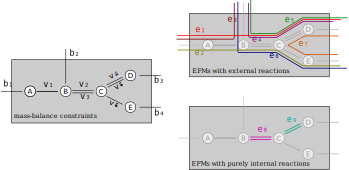
\includegraphics[width=0.8\textwidth]{toy1}
	\caption{A toy example with 6 internal reactions and 4 exchange reactions. The flux cone is spanned by 9 EFMs.}\label{fig:toy1}
	\end{center}
\end{figure}

EFMs are closely related to Extreme Pathways (EPs) and distinguishing them requires more subtle definitions. For further reading you can refer to \cite{klamt_two_2003}.

\subsubsection{Classification of EFMs}
Even in our small toy example in Figure \ref{fig:toy1}, we already encounter a common problem that arises when dealing with EFMs -- i.e. cycles. In this example, it's quite obvious that the two EFMs that consist of combining two opposing reactions is futile and should be ignored. Larger networks, however, might have much larger cycles that are harder to identify and get rid of.

First, we need to distinguish between \textit{primary exchange} and \textit{currency exchange} reactions. The former are the standard reactions that exchange nutrients between the cell/compartment and its environment (sugar import, CO$_2$ export, etc.). \textit{Currency exchange} reactions do not, in fact, exchange material between compartments, but are rather abstract representations of energy dissipation. A canonical example would be the ATP maintenance reaction that is present in most metabolic models: ATP + H$_2$O $\rightharpoonup$ ADP + P$_i$.

Now, we can define the three types of EFMs (\cite{price_extreme_2002}, see Figure \ref{fig:efm_types}):
\begin{description}
	\item[I] -- \textit{Primary systemic EFMs} have at least one active primary exchange flux.
	\item[II] -- \textit{Futile cycles} have no active primary exchange fluxes, and at least one active currency exchange flux.
	\item[III] -- \textit{Internal cycles} have no active exchange fluxes (neither primary nor currency). 
\end{description}

\begin{figure}[ht!]
	\begin{center}	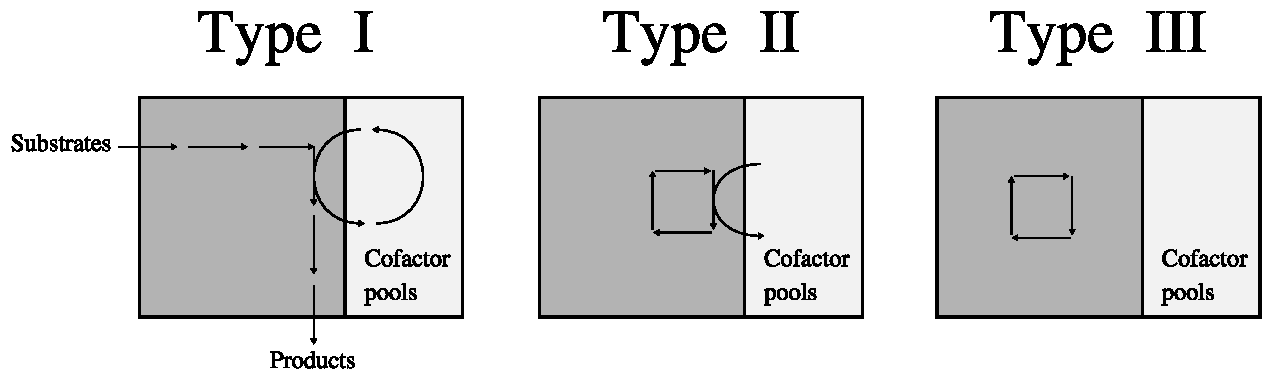
\includegraphics[width=0.7\textwidth]{extreme_pathway_types}
	\caption{The three types of Elementary Flux Modes.}\label{fig:efm_types}
	\end{center}
\end{figure}

To illustrate the three types of pathways, we present another toy model with one currency exchange reaction and two primary exchange reactions (Figure \ref{fig:toy2}). This model contains all the three types of EFMs.
\begin{figure}[ht!]
	\begin{center}
	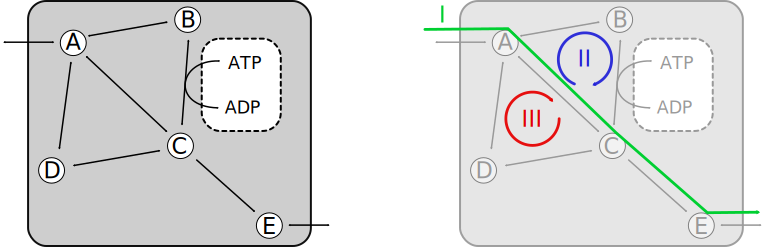
\includegraphics[width=0.5\textwidth]{toy2}
	\caption{A small toy model with 8 internal reactions, 2 primary exchange reactions, and one currency exchange reaction. In this simple network, one can identify all three types of extreme pathways. The Type I pathway (green) is typically the type of solution that most constrain-based models are seeking. The Type II pathway ($A \rightarrow B \rightarrow C \rightarrow A$, blue) is a typical futile cycle, since it does not involve any primary exchange reactions, but does \emph{waste} ATP. The Type III pathway ($A \rightarrow C \rightarrow D \rightarrow A$, red) is called internal since none of its reactions are exchange reactions. An internal cycle will never be thermodynamically feasible.
	}\label{fig:toy2}
	\end{center}
\end{figure}

In the next section, we will see how this three type classification is useful to separate thermodynamically feasible pathways from infeasible ones.

\subsection{Thermodynamics}\label{sec:thermodynamics}
A fundamental principle in enzymatic catalysis is the notion that enzymes can accelerate the rate of a reaction, but not change its thermodynamic equilibrium, therefore they have no effect on the \textit{direction} of flux.

\subsubsection{The Gibbs free energy of reaction}

The second law of thermodynamics states that entropy can never decrease over time in an isolated system. In living cells, which are open systems in constant pressure, temperature, and pH, entropy can be replaced by the concept of transformed Gibbs free energy of reaction \cite{alberty_biochemical_2006-1}, denoted $\Delta_r G'$. Then, for a chemical reaction to be feasible, it must impose a negative change in $\Delta_r G'$:
\begin{eqnarray}
\Delta_r G' < 0
\end{eqnarray}
For the purpose of constraint-based modeling, it is enough to understand how each $\Delta_r G'$ is affected by its reactant concentration. We typically use the assumption that biochemical reactions occur in dilute aqueous solutions (i.e. the activity coefficient of uncharged species is unity). In this case, the transformed Gibbs free energy of reaction $j$ is given by:
\begin{eqnarray}\label{eq:thermo1}
\Delta_r G'_j &=& \Delta_r G'^\circ_j + R\,T\cdot\ln(Q'_j) \\
Q'_j &=& \prod_i c_i^{S_{ij}}
\end{eqnarray}
where $R$ is the gas constant, $T$ is the temperature (in Kalvin), $Q'$ is the biochemical reaction quotient, $c_i$ is the molar concentration of a reactant (substrate of product) and $S_{ij}$ are the corresponding stoichiometric coefficients (i.e. a row in $\stoichmatint$). $\Delta_r G'^\circ_j$ represents that $\Delta_r G'_j$ in standard conditions, which is typically defined as 1 M for each one of the reactants. One way to measure $\Delta_r G'^\circ_j$, is to let the reaction run until it reaches equilibrium, and measure the concentrations of all reactants. The value of $Q'$ in equilibrium is called the \textit{equilibrium constant} and is denoted $K'$. Also, since know that at equilibrium $\Delta_r G'_j = 0$, we can solve for $\Delta_r G'^\circ_j$ and get:
\begin{eqnarray}
\Delta_r G'^\circ_j &=& -R\,T\cdot\ln(K'_j)
\end{eqnarray}
For further reading on thermodynamics of biochemical reactions, see \cite{alberty_recommendations_2011, noor_note_2013}.


Finally, we would like to rewrite equations \ref{eq:thermo1} in a more convenient way that corresponds well with our linear algebra notation. First, one can notice that taking the log from $Q'$ makes it a linear function of the log-concentration values: $\ln(Q'_j) = \sum_i S_{ij} \cdot \ln(c_i)$. In addition, from now on we will use a matrix notation for calculating the vector of all reaction Gibbs energies ($\myvector{\Delta_r G'}$):
\begin{eqnarray}
\myvector{\Delta_r G'} = \myvector{\Delta_r G'^\circ} + R\,T\cdot\stoichmat^\top \myvector{x}
\end{eqnarray}
where we define $\myvector{x}$ as the vector of log-concentrations, i.e. $x_i = \ln(c_i)$.

\subsubsection{Irreversibility is an approximation}
In pure physics terms, every chemical reaction should be reversible. There are cases, where the equilibrium is so far from unity, which makes it impossible for the reaction to reach equilibrium in practice. In these cases, it is sometimes convenient to assume that the reaction is irreversible and complete ignore the reverse direction. In defining the flux cone, this assumption can significantly reduce the solution space and number of EFMs.

Most thermodynamics-aware models, however, cannot make this assumption. Every reaction must have a defined equilibrium constant, no matter how extreme it might be. Therefore, from now on, we assume $\Delta_r G'^\circ_j$ has a finite value, even for reactions that are defined as irreversible in our model. There is no universal threshold for $\Delta_r G'^\circ_j$ which make a reaction irreversible. It is context dependent and a topic of much debate \cite{mavrovouniotis_identification_1993-1, henry_thermodynamics-based_2007, noor_integrated_2012}. 

Beyond $\Delta_r G'^\circ_j$, probably the most important parameters for determining the reversibility are the range of concentrations allowed for each of the reactants. Basically, a reversible reaction should have both positive and negative values to its $\Delta_r G'_j$, depending on the chosen reactant concentrations within their predefined ranges. If we denote the vectors of lower and upper bounds as $\myvector{b}^L$ and $\myvector{b}^U$, respectively, the constraint on $\myvector{x}$ would be:
\begin{eqnarray}
\ln(\myvector{b}^L) \leq \myvector{x} \leq \ln(\myvector{b}^U)
\end{eqnarray}
It is easy to see, that the lowest value for $\Delta_r G'_j$ is achieved when all substrate concentrations are set to their value in $\myvector{b}^U$, and all product concentrations to $\myvector{b}^L$. The highest value of $\Delta_r G'_j$ occurs in the opposite extreme. Then, it become straightforward to check if a reaction is, by itself, reversible or not.

\subsubsection{Thermodynamic Feasibility of EFMs}
Given a specific elementary flux mode $\myvector{e}^j$ (or any flux vector $\myvector{v}$, for that matter), we would like to know whether it is thermodynamically feasible according to the second law. First, every one of the support reactions must be feasible in the direction defined by $\myvector{e}^j$. However, the same metabolite can be a substrate for one reaction, and a product for another and therefore there is inter-dependence between the $\Delta_r G'_j$ values of these reactions. Sometimes, even though a series of reactions can be individually feasible, their combination is infeasible. This has been termed a \textit{distributed bottleneck} by \textcite{mavrovouniotis_identification_1993-1} in 1993.

Using Linear Programming, it is relatively simple to test thermodynamic feasibility:
\begin{eqnarray}\label{eq:feasible_lp}
\textsf{Find}&\myvector{x}&\nonumber\\
\textsf{such that}&&\nonumber\\
\myvector{\Delta_r G'} &\equiv& \myvector{\Delta_r G'^\circ} + RT \cdot \stoichmat^\top \myvector{x} \nonumber\\
\myvector{\Delta_r G'} &<& 0\nonumber\\
\ln(\myvector{b}^L) &\leq& \myvector{x} ~\leq~ \ln(\myvector{b}^U) 
\end{eqnarray}

\subsubsection{Max-min Driving Force}
In order to provide a more quantitative measure for the thermodynamic feasibility of a given pathway, the Max-min Driving Force (MDF) method provides a relatively simple measure. We adjust the Linear Program in Equation \ref{eq:feasible_lp}, by adding a margin variable ($B$) and maximizing its value:
\begin{eqnarray}
\textsf{MDF} &\equiv& \max_{B,\myvector{x}}{B} \nonumber\\
\textsf{such that}&&\nonumber\\
\myvector{\Delta_r G'} &\equiv& \myvector{\Delta_r G'^\circ} + RT \cdot \stoichmat^\top \myvector{x} \nonumber\\
\myvector{\Delta_r G'} &<& -B\nonumber\\
\ln(\myvector{b}^L) &\leq& \myvector{x} ~\leq~ \ln(\myvector{b}^U) 
\end{eqnarray}
If the MDF is positive, then there exists a set of concentrations $\myvector{x}$ (inside the allowed range) such that $\myvector{\Delta_r G'} \leq -B < 0$, i.e. this pathway is thermodynamically feasible. The larger $B$ is, the ``more feasible'' it is, since we can keep all reactions farther away from equilibrium. From non-equilibrium thermodynamic theory, we know that reactions that are far from equilibrium tend to be more efficient (as described by the flux-force relationship \cite{beard_relationship_2007-1}). An example for MDF calculation is given in Figure \ref{fig:mdf}.

An online interface for running MDF analysis can be found here: \url{http://equilibrator.weizmann.ac.il/pathway/}.

\begin{figure}[ht!]
	\begin{center}
		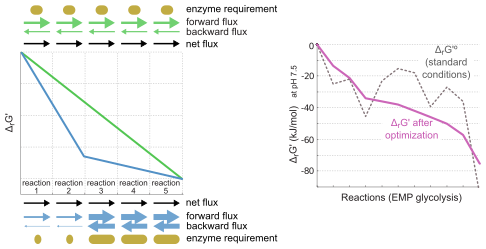
\includegraphics[width=0.8\textwidth]{mdf}
		\caption{(left) Schematic comparison between two pathways. Each pathway starts and ends with the same compounds, employs five enzymes and carries the same net flux. The kinetic parameters of all enzymes in both pathways, as well as enzyme and metabolite concentrations, are assumed to be identical. (right) Energetic profile of Embden-Meyerhof-Parnas glycolysis. Dashed black line corresponds to $\Delta_r G'^\circ$ values (metabolite concentrations of 1M) of pathway reactions at pH 7.5. Red line corresponds to $\Delta_r G'$ values of pathway reactions after an optimization procedure that maximizes the driving force of the thermodynamic bottleneck reactions. Figure is from \textcite{noor_pathway_2014}.
		}\label{fig:mdf}
	\end{center}
\end{figure}

\subsubsection{Thermodynamic Flux Balance Analysis (TFBA)}

Thermodynamic FBA (also known as Thermo\-dynamic-based Metabolic Flux Analysis \cite{henry_thermodynamics-based_2007}) was designed to deal with thermodynamically infeasible flux solutions within the framework of FBA:
\begin{eqnarray}
\textsf{\textbf{FBA}} && \nonumber\\
\myvector{v^*} &=& \mathrm{arg\max_v} {~\myvector{c}^\top\myvector{v}}\nonumber\\
\textsf{such that:} && \nonumber\\
\stoichmatint \myvector{v} &=& \myvector{0}  \label{eq:fba1} \\
\myvector{v}_{LB} &\leq& \myvector{v} ~\leq~ \myvector{v}_{UB} \label{eq:fba2}
\end{eqnarray}
where $\myvector{c} \in \mathbb{R}^r$ is the objective function, and the constants are the internal stoichiometric matrix $\stoichmatint \in \mathbb{R}^{m \times r}$. $\myvector{v}_{LB}$ and $\myvector{v}_{UB}$ are the lower and upper bounds on the fluxes, typically relevant only for exchange fluxes.

TFBA adds another two sets of variables -- the boolean flux indicators ($\myvector{y} \in \{0, 1\}^r$), and the log-concentrations ($\myvector{x} \in \mathbb{R}^r$). Then, the following constraints are added to the Linear Problem (which is now actually a Mixed-Integer Linear Problem -- MILP):
\begin{eqnarray}
\textsf{\textbf{TFBA}} && \nonumber\\
\myvector{v^*} &=& \mathrm{arg\max_v} {~\myvector{c}^\top\myvector{v}}\nonumber\\
\textsf{such that:} && \nonumber\\
\stoichmatint \myvector{v} &=& \myvector{0} \nonumber\\
\myvector{v}_{LB} &\leq& \myvector{v} ~\leq~ \myvector{v}_{UB} \nonumber\\
0 &\leq& M \myvector{y} - \myvector{v} ~\leq~ M  \label{eq:tfba1}\\
0 &<& M \myvector{y} + \myvector{\Delta_r G'} ~<~ M \label{eq:tfba2} \\
\myvector{\Delta_r G'} &=& \myvector{\Delta_r G'^\circ} + RT \cdot \stoichmat^\top \myvector{x} \label{eq:tfba3}\\
\ln(\myvector{b}^L) &\leq& \myvector{x} ~\leq~ \ln(\myvector{b}^U) \label{eq:tfba4}
\end{eqnarray}
The new constants are the vector of standard Gibbs energies of reaction $\myvector{\Delta_r G'^\circ}$ (in units of kJ/mol), the gas constant $R$ = 8.31 J/mol/K and temperature $T$ = 300 K. $M$ which is a very large number (larger than any of the possible flux and Gibbs free energy). Note also the difference between the internal stoichiometric matrix ($\stoichmatint$) used for the pseudo steady-state assumption, versus the full stoichiometric matrix ($\stoichmat$) used in the Gibbs free energy calculation.

Equations \ref{eq:tfba3}-\ref{eq:tfba4} should be familiar, and are exactly the same as in previous sections. To understand how the other two constraints (\ref{eq:tfba1}-\ref{eq:tfba2}) enforce thermodynamic feasibility, we consider three possible cases for each reaction $j$ separately:
\begin{enumerate}
	\item $v_j > 0$ : the only possible value that $y_j$ can have is 1, otherwise, $My_j - v_j$ would be negative and violate constraint \ref{eq:tfba1}. Therefore, constraint \ref{eq:tfba2} becomes $0 < M + \Delta_r G'_j < M$, which means that $\Delta_r G'_j < 0$.
	\item $v_j < 0$ : the only possible value that $y_j$ can have is 0, otherwise, $My_j - v_j$ would be larger than $M$ and violate constraint \ref{eq:tfba1}. Therefore, constraint \ref{eq:tfba2} becomes $0 < \Delta_r G'_j < M$, which means that $\Delta_r G'_j > 0$.
	\item $v_j = 0$ : both $0$ and $1$ are possible solutions for $y_j$. Therefore, there are no constraints on $\Delta_r G'_j$.
\end{enumerate}
Summarizing these 3 cases, one can concisely write:
\begin{eqnarray}
\forall j:v_j = 0~\vee~\text{sign}(v_j) = -\text{sign}(\Delta_r G'_j)\,,
\end{eqnarray}
which is exactly the second law of thermodynamics.

\subsubsection{Loopless Flux Balance Analysis (ll-FBA)}
The loopless algorithm \cite{schellenberger_elimination_2011} is very similar to TFBA, except that there are no actual thermodynamic values. This way, thermodynamically infeasible internal (Type III) cycles are eliminated, while all other pathways are kept \cite{noor_proof_2012}. The set of equations describing ll-FBA are:
\begin{eqnarray}
\textsf{\textbf{ll-FBA}} && \nonumber\\
\myvector{v^*} &=& \mathrm{arg\max_v} {~\myvector{c}^\top\myvector{v}}\nonumber\\
\textsf{such that:} && \nonumber\\
\stoichmatint \myvector{v} &=& \myvector{0} \label{eq:llfba1} \\
\myvector{v}_{LB} &\leq& \myvector{v} ~\leq~ \myvector{v}_{UB} \\
0 &\leq& M \myvector{y} - \myvector{v} ~\leq~ M
\label{eq:llfba2} \\
0 &<& M \myvector{y} + \myvector{\Delta_r G'} ~<~ M \label{eq:llfba3} \\
\myvector{\Delta_r G'} &\in& \ker{(\stoichmat)}^\perp \label{eq:llfba5}
\end{eqnarray}
here, $\myvector{\Delta_r G'}$ is not constrained by the $\myvector{\Delta_r G'}^\circ$ and the metabolite concentrations, but is only required to be orthogonal to the null-space of $\stoichmat$ (or, equivalently, to be in $\mathrm{image}(\stoichmat^\top)$).

Why does ll-FBA not eliminate type II cycles from the set of flux solutions? These futile cycles ``waste'' resources such as ATP, but are thermodynamically feasible. They are only considered ``cycles'' because we chose to give co-factors a special status (namely, they are external metabolites that do not need to be kept at steady-state). In other words, type II EFMs are in the null-space of $\stoichmatint$, but not in the null-space of $\stoichmat$ (just like type I EFMs). Therefore, it is possible to assign negative $\Delta_r G'$ values to all reactions in a type II EFMs.

Interestingly, this argument can be applied also to the reverse of such futile cycle. Running a futile cycle in reverse is sometimes called an Energy Generating Cycle (EGC), and is obviously unrealistic. Furthermore, unlike type III cycles that do not affect the biomass rate in standard FBA, EGCs have the potential to increase the maximal biomass yield and pose a more serious problem in FBA models \cite{fritzemeier_erroneous_2017-2}. This is one of the cases where TFBA differs from ll-FBA, as it prevents the use of EGCs completely, while ll-FBA doesn't.

\subsection{Metabolic engineering algorithms}

\subsubsection{Phenotypic Phase Plane (PPP)}
This useful concept derived from FBA, is a term for 2D projections on the flux polytope. Typically, one chooses specific reaction (e.g. exchange of succinate) for the y-axis and the FBA objective (i.e. biomass rate) for the x-axis. The projection of the flux polytope onto this plane creates a convex polygon shape and helps to visualize how important a certain flux is for creating biomass. Often for cases where the selected flux is a fermentation product, the PPP is referred to as a \textit{production envelope}. It is standard practice to present strain-design results by overlaying two or more PPPs, e.g. a knockout strain versus the wild-type (Figure \ref{fig:ppp}). Using such comparisons, it is easy to see if the knockout is useful for forcing a cell to produce the desired chemical byproduct, by coupling its production to the biomass rate.

\begin{figure}[ht!]
	\begin{center}
		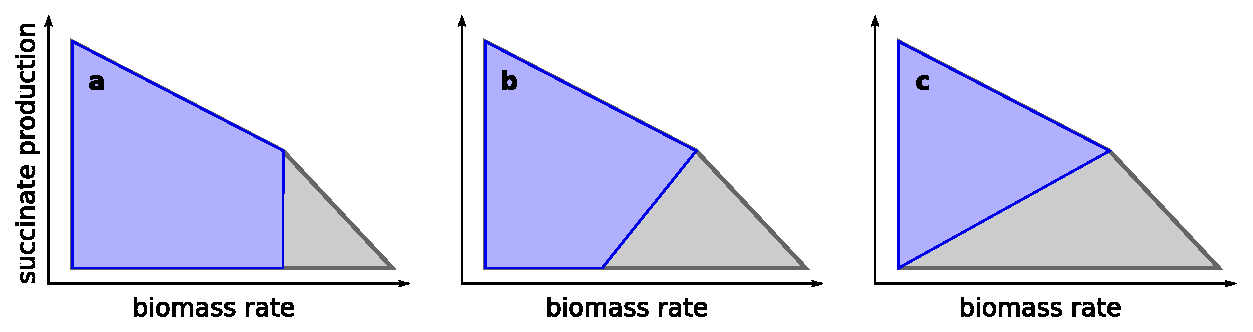
\includegraphics[width=0.7\textwidth]{ppp}
		\caption{Phenotypic phase planes for anaerobic succinate production from glucose based on the \textit{E. coli} core model. (a) wild-type strain (light gray) vs. triple-deletion mutant (ACKr, ATPS4r, FUM) resulting in a design without growth-coupling (purple). (b) wild-type strain vs. triple-deletion mutant (ACALD, PYK, ME2) resulting in a partially growth-coupled design. (c) wild-type strain vs. double-deletion mutant (ACALD, LDH\_D) resulting in a fully growth-coupled design. Figure is from \textcite{machado_co-evolution_2015}.}\label{fig:ppp}
	\end{center}
\end{figure}

\subsubsection{OptKnock and its derivatives}
\textcite{burgard_optknock_2003-1} phrased the OptKnock optimization problem first as a bi-level mixed-integer linear optimization problem. The inner problem is standard FBA, maximizing an objective function $\myvector{c}_\textsf{in}^\top \myvector{v}$. This encodes the assumption that each knockout strain we consider for the outer problem, evolves to maximize the objective (which is typically set to be the biomass function). Then, we choose the one knockout that maximizes the outer objective $\myvector{c}_\textsf{out}^\top \myvector{v}$ -- typically the secretion rate of the desired product (e.g. succinate).
\begin{eqnarray}
\textsf{\textbf{OptKnock}} && \nonumber\\
\max_{\myvector{y}}~~\myvector{c}_{\textsf{out}}^\top \myvector{v}&&\nonumber\\
\textsf{subject to}&&\nonumber\\
&\max_{\myvector{v}}~\myvector{c}_{\textsf{in}}^\top \myvector{v}&\nonumber\\
&\textsf{subject to}&\nonumber\\
&&\stoichmatint \myvector{v} = \myvector{0} \nonumber\\
&&v_{\textsf{LB},\,j} \cdot y_j \leq v_j \leq y_j \cdot v_{\textsf{UB},\,j} \nonumber\\
&\myvector{y} \in \{0, 1\}^r \nonumber\\
&\sum_j{(1-y_j)} \leq K & \label{eq:optknock}
\end{eqnarray}
where, $K$ is the maximum number of allowed knockouts. The inner LP is a standard FBA optimization problem, except that a few of the reactions are ``knockout out'' -- when a reaction indicator is set to 0 by the external LP it forces the corresponding flux to zero, i.e. $y_j = 0 \rightarrow v_j = 0$. In addition, we set $v_{\textsf{LB},\,biomass} > 0$ and $y_{biomass} = 1$, since we only want to consider mutants that show at least some minimal growth. Finally, the external LP places an upper bound on the total number of knockouts, which is useful for two reasons: (1) making sure we don't have too many knockouts that would make the genetic manipulation impractical, and (2) to reduce the computational load required to solve the MILP. Nevertheless, even for small $K$, solving the bi-level MILP  directly is not tractable for large networks (such as the genome-scale \textit{E. coli} model). Fortunately, \textcite{burgard_optknock_2003-1} provided a solution, by converting into a single-level MILP using duality theory.

The dual of the inner optimization problem in \ref{eq:optknock} is:
\begin{eqnarray}
\min_{\myvector{\lambda},\myvector{\mu},\myvector{\omega}} ~\sum_j y_j (v_{\textsf{UB},\,j} \cdot \mu_j - v_{\textsf{LB},\,j} \cdot \omega_j)&\nonumber\\
\textsf{subject to}&\nonumber\\
&\stoichmatint^\top \myvector{\lambda} + \myvector{\mu} - \myvector{\omega} \geq \myvector{c}_\textsf{in} \nonumber\\
&\myvector{\mu}, \myvector{\omega} \geq 0\,.
\end{eqnarray}
Since duality theory states if the optimums solutions of the primal and dual problems are bounded, their objective function values must be equal to one another, so ensuring optimality can be achieved by equating the two objectives: $\myvector{c}_\textsf{in}^\top \myvector{v} = \sum_j y_j (v_{\textsf{UB},\,j} \cdot \mu_j - v_{\textsf{LB},\,j} \cdot \omega_j)$. However, using this equation as a constraint in the outer optimization problem would make it non-linear, since it contains products of two variables ($y_j \cdot \mu_j$ and $y_j \cdot \omega_j$). We can, however, use the fact that $y_j$ are binary in order to cast this expression into a linear form.

First, we introduce a new set of auxiliary variables $\myvector{m} \in \mathbb{R}^r$, and constrain them to be $m_j = y_j \cdot \mu_j$ by adding the following:
\begin{eqnarray}
	0 \leq &m_j& \leq y_j \cdot M \nonumber\\
	\mu_j - (1 - y_j) \cdot M \leq &m_j& \leq \mu_j\,.
\end{eqnarray}
As before, $M$ is a constant larger than any possible value of $\mu_j$. Considering the two cases for $y_j$, one can easily see that $y_j = 0 ~\rightarrow~ m_j = 0$ and $y_j = 1 ~\rightarrow~ m_j = \mu_j$, which is what we wanted to achieve. We do exactly the same for $\myvector{\omega}$ and another set of variables $\myvector{u} \in \mathbb{R}^r$. Then we can rewrite the dual objective as: $\sum_j y_j (v_{\textsf{UB},\,j} \mu_j - v_{\textsf{LB},\,j} \omega_j) = \myvector{v}_\textsf{UB}^\top \myvector{m} - \myvector{v}_\textsf{LB}^\top\myvector{u}$.

Using this notion, we get a single-level MILP problem for OptKnock:
\begin{eqnarray}\label{eq:optknock2}
\textsf{\textbf{OptKnock}} & \nonumber\\
\max_{\myvector{y},\myvector{v},\myvector{\lambda},\myvector{\mu},\myvector{\omega},\myvector{m},\myvector{u}}~~\myvector{c}_\textsf{out}^\top \myvector{v}&\nonumber\\
\textsf{subject to}&\nonumber\\
&\stoichmatint \myvector{v} = \myvector{0} \nonumber\\
&v_{\textsf{LB},\,j} \cdot y_j \leq v_j \leq y_j \cdot v_{\textsf{UB},\,j} \nonumber\\
&\myvector{c}_\textsf{in}^\top \myvector{v} = \myvector{v}_\textsf{UB}^\top \myvector{m} - \myvector{v}_\textsf{LB}^\top\myvector{u} \nonumber\\
&\myvector{c}_\textsf{in} \leq \stoichmatint^\top \myvector{\lambda} + \myvector{\mu} - \myvector{\omega} \nonumber\\
&0 \leq \myvector{\mu}, \myvector{\omega} \nonumber\\
&0 \leq \myvector{m} \leq \myvector{y} \cdot M \nonumber\\
&\myvector{\mu} - (1 - \myvector{y}) \cdot M \leq \myvector{m} \leq \myvector{\mu} \nonumber\\
&0 \leq \myvector{u} \leq \myvector{y} \cdot M \nonumber\\
&\myvector{\omega} - (1 - \myvector{y}) \cdot M \leq \myvector{u} \leq \myvector{\omega} \nonumber\\
&\sum_j{(1-y_j)} \leq K  
\end{eqnarray}

\subsubsection{Derivatives of OptKnock}

A comprehensive review by \textcite{machado_co-evolution_2015} lists the many published algorithms for \textit{in silico} strain design that followed after OptKnock (see Figure \ref{fig:optknock_derivatives}).
\begin{figure}[ht!]\label{fig:optknock_derivatives}
	\begin{center}
		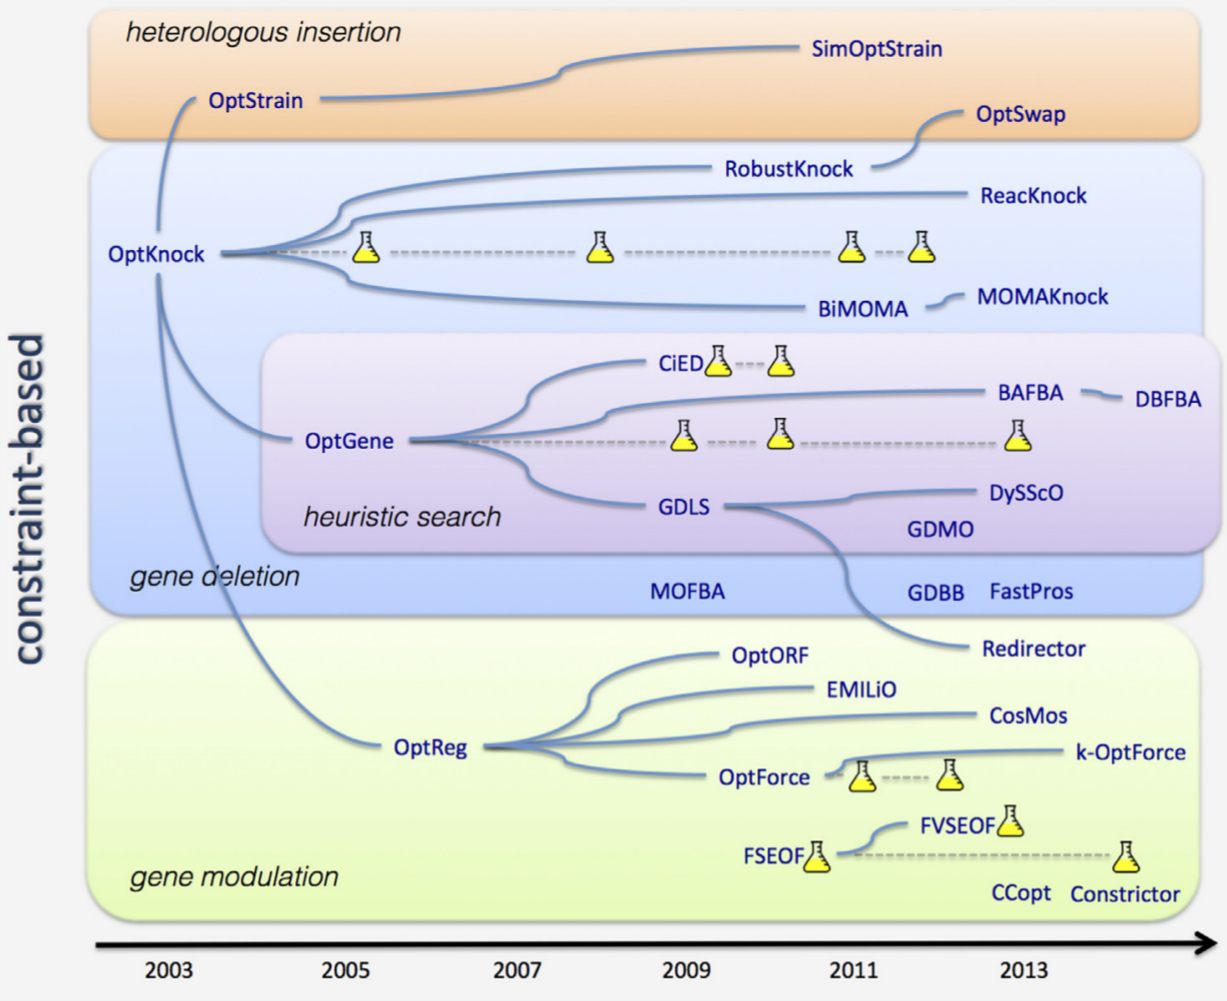
\includegraphics[width=0.75\textwidth]{optknock_derivatives.png}
	\end{center}
	\caption{A timeline of all constraint-based strain design methods that followed OptKnock (figure is from \cite{machado_co-evolution_2015}).}
\end{figure}

Robust\-Knock is an improvement for Opt\-Knock, introduced by \textcite{tepper_predicting_2010-1} in 2010, which accounts for competing pathways that might reduce the chemical production rates. One common issue with standard Opt\-Knock, is that it only looks at the maximal rate of the chemical production rate: $\max \myvector{c}_\textsf{out}^\top \myvector{v}$. However, as visualized by the production envelope in Figure \ref{fig:ppp}a, there might be redundancy in the solution space, where the same biomass rate can be achieved without any production of the desired chemical. Robust\-Knock addresses this problem by performing a max-min optimization, i.e. maximizing the lowest value of $\myvector{c}_\textsf{out}^\top \myvector{v}$ over all $\myvector{v}$ that satisfy the inner LP. This method yields solutions like in Figure \ref{fig:ppp}b-c.

\printbibliography

\end{document}

